\documentclass[tikz, border=10pt]{standalone}
\usetikzlibrary{shapes.geometric, arrows.meta, positioning, shadows}

\begin{document}
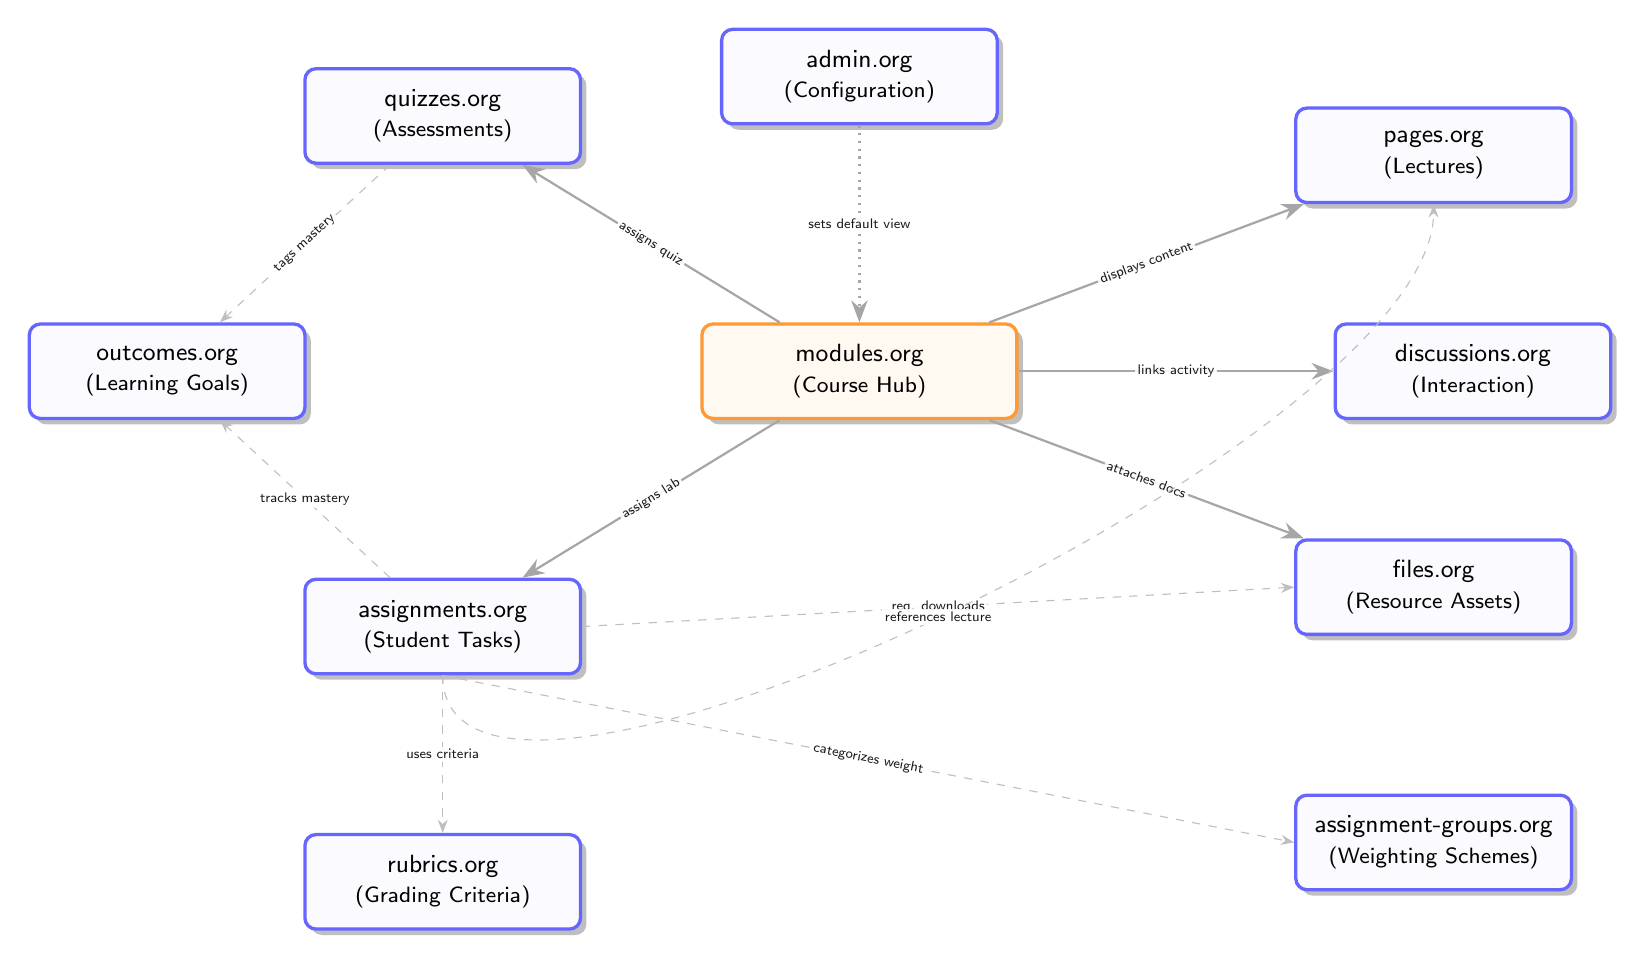
\begin{tikzpicture}[
    file/.style={
        rectangle, 
        draw=blue!60, 
        fill=blue!2, 
        very thick, 
        minimum width=3.5cm, 
        minimum height=1.2cm, 
        align=center, 
        rounded corners,
        drop shadow,
        font=\sffamily\small
    },
    hub/.style={
        file, 
        draw=orange!80, 
        fill=orange!5,
        minimum width=4cm
    },
    link/.style={
        -{Stealth[scale=1.2]}, 
        thick, 
        draw=gray!70
    },
    secondary_link/.style={
        -{Stealth[scale=1.0]}, 
        dashed, 
        draw=gray!50
    },
    label_text/.style={
        font=\sffamily\tiny,
        fill=white,
        inner sep=1pt,
        opacity=0.9
    }
]

    % CENTRAL HUB
    \node[hub] (modules) {modules.org \\ \footnotesize (Course Hub)};

    % CONTENT COLUMN (Right Side)
    \node[file] (pages) [above right=1.5cm and 3.5cm of modules] {pages.org \\ \footnotesize (Lectures)};
    \node[file] (discussions) [right=4cm of modules] {discussions.org \\ \footnotesize (Interaction)};
    \node[file] (files) [below right=1.5cm and 3.5cm of modules] {files.org \\ \footnotesize (Resource Assets)};

    % ASSESSMENT & CONFIG (Left/Bottom Side)
    \node[file] (quizzes) [above left=2cm and 1.5cm of modules] {quizzes.org \\ \footnotesize (Assessments)};
    \node[file] (assignments) [below left=2cm and 1.5cm of modules] {assignments.org \\ \footnotesize (Student Tasks)};
    \node[file] (admin) [above=2.5cm of modules] {admin.org \\ \footnotesize (Configuration)};

    % SUPPORTING METADATA (Outliers)
    \node[file] (outcomes) [left=5cm of modules] {outcomes.org \\ \footnotesize (Learning Goals)};
    \node[file] (rubrics) [below=2cm of assignments] {rubrics.org \\ \footnotesize (Grading Criteria)};
    \node[file] (groups) [below=2cm of files] {assignment-groups.org \\ \footnotesize (Weighting Schemes)};

    % PRIMARY LINKS FROM MODULES
    \draw[link] (modules) -- (pages) node[midway, label_text, sloped] {displays content};
    \draw[link] (modules) -- (discussions) node[midway, label_text] {links activity};
    \draw[link] (modules) -- (files) node[midway, label_text, sloped] {attaches docs};
    \draw[link] (modules) -- (quizzes) node[midway, label_text, sloped] {assigns quiz};
    \draw[link] (modules) -- (assignments) node[midway, label_text, sloped] {assigns lab};
    \draw[link, dotted] (admin) -- (modules) node[midway, label_text] {sets default view};

    % SECONDARY LINKS FROM ASSIGNMENTS
    \draw[secondary_link] (assignments) -- (outcomes) node[midway, label_text] {tracks mastery};
    \draw[secondary_link] (assignments) -- (rubrics) node[midway, label_text] {uses criteria};
    \draw[secondary_link] (assignments.east) -- (files.west) node[midway, label_text] {req. downloads};
    \draw[secondary_link] (assignments.south) -- (groups.west) node[midway, label_text, sloped] {categorizes weight};
    
    % Curve assignment->pages to avoid modules hub
    \draw[secondary_link] (assignments.south) .. controls +(down:3cm) and +(down:3cm) .. (pages.south) 
        node[midway, label_text] {references lecture};

    % QUIZ LINKS
    \draw[secondary_link] (quizzes) -- (outcomes) node[midway, label_text, sloped] {tags mastery};

\end{tikzpicture}
\end{document}
